\documentclass[12pt]{article}

% Language setting
\usepackage[utf8]{inputenc}
\usepackage[bulgarian]{babel}

% --------------------- Packages  --------------------
% Use biblatex
\usepackage{biblatex}
\addbibresource{bibliography.bib}
% Table thickness
\usepackage{ctable}
% Equations: SI units
\usepackage{siunitx}
% Approximately equal
\usepackage{amssymb}
% degrees symbol
\usepackage{gensymb}
% warning box
\usepackage{pifont,mdframed}

\newenvironment{warning}
  {\par\begin{mdframed}[linewidth=2pt, linecolor=white]%
    \begin{list}{}{\leftmargin=1cm
                   \labelwidth=\leftmargin}\item[\Large\ding{43}]}
  {\end{list}\end{mdframed}\par}

% --------------------- Title  --------------------
\addbibresource{bibliography.bib}
\title{Косвено измерване на обем на тяло}
\author{Виолета Кабаджова}
\date{October 2022}

\begin{document}

% Anfang der Titelseite________________________________________________________________________________
\begin{titlepage}
	\flushleft
% 	\begin{center}
	%{\scshape\Large Werkstoffe III \hspace{2.5cm} Laborbericht \hspace{2.5cm}HS 2022 \par}
	{\scshape\Large Протокол III \hspace{2cm} Механика - практикум\par}
	\vspace{5cm}
	{\huge\bfseries Закон за запазване на импулса. Централен удар на сфери\par}
	\vspace{1cm}
	{\LARGE\bfseries Лабораторно упражнение №3\par}
	\vspace{5cm}
    % {\LARGE\bfseries Физически Факлутет към Софийски Университет ``Св. Климент Охридски \par}
    {\LARGE\bfseries Виолета Кабаджова, \par}
%   {\LARGE\bfseries Group: X\par}
    {\large\bfseries ККТФ, факл. номер: 3PH0600026\par}
	\vspace{1cm}
	
	{\large Физически Факлутет, 
	
	Софийски Университет "Св. Климент Охридски"
	
	6 ноември 2022 г.\par}
	
\end{titlepage}

\section{Теоритична част}
\subsection{Закон за Запазване на Импулса (ЗЗИ)}
Законът за запазване на импулса гласи: 
\begin{warning}
В изолирана система от две или повече тела сумарният импулс \(\vec{p} = \sum_{i=1}^{N}{\vec{p_i}}\) не се променя с времето, т.е. \(\vec{p} = const\). При различни вътрешни взаимодействия може да става само преразпределението му между телата на системата.
\end{warning}

Изразено от горното втория закон на Нютон придобива вида:
\begin{equation}
    \vec{F} = \frac{d\vec{p}}{dt} = \frac{d(m\vec{v})}{dt},
\end{equation}

където \(\vec{F}\) представлява резултатната сила, действаща на тялото или на системата. 

\subsection{Коефициент на възстановяване на скоростта}\label{sec:coefficient-of-restitution}
Един от широко разпространените методи за експериментално изследване на ЗЗИ е чрез удари на тела. Мигновено след удара телата имат различни скорости \((\vec{u_1}, \vec{u_2})\) спрямо скоростите преди момента на удара \((\vec{v_1}, \vec{v_2})\). Количествената мярка за проните в скоростите на телата и вида на удара се нарича коефициент на възстновяване на скоростта К, изразяващ се по следния начин:

\begin{equation}\label{eq:coefficient_of_restitution}
    K = \frac{|u_2 - u_1|}{|v_2 - v_1|}
\end{equation}


\subsection{Деформация при удар}
Механичното взаимодействие при удар между реални тела протича в интервал от време \(\tau = t_2 - t_1\) от порядъка на \(10^{-2}\) до \(10^{-6}\) s. В този период телата изпитват някакъв вид деформация - пластична (такава при кото след удара телата се движат като едно цяло: \(\vec{u_1} = \vec{u_2}\)) и еластична (такава, която е изцяло обратима). От формула \ref{eq:coefficient_of_restitution} следва, че идеално пластичен удар би имало коефициент K=0, а идеално еластичен К=1. Съответно за реални тела коефициентът К би приемал стойности 0 < K < 1.

От ЗЗИ следва, че:

\begin{equation}
    \vec{p_0} = m_1\vec{v_1} + m_2\vec{v_2} = m_1\vec{u_1} + m_2\vec{u_2} = \vec{p_\tau} 
\end{equation}

\section{Експериментална част}
\subsection{Експериментална установка}\label{sec:experimental-setup}
\begin{figure}
    \centering
    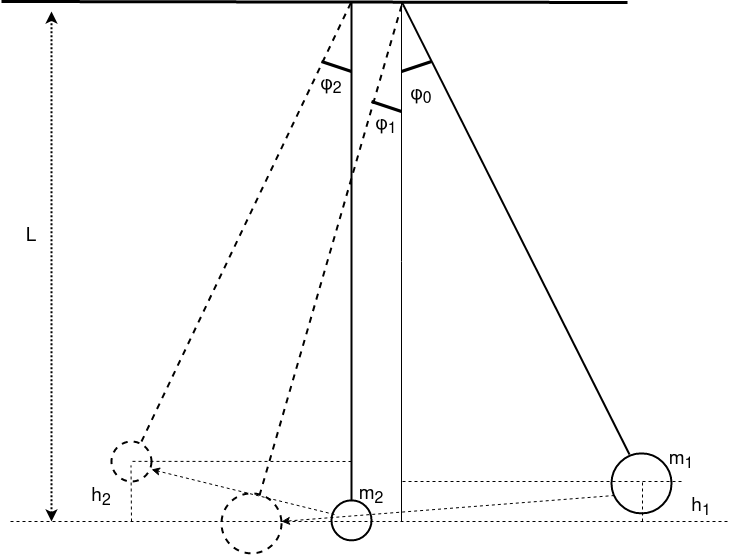
\includegraphics[width=\textwidth]{images/spehres-momentum-conservation-law.drawio.png}
    \caption{Експериментална установка}
    \label{fig:setup}
\end{figure}

На фиг. \ref{fig:setup} е показана експерименталната установка. Тя се състои от две сфери с различни маси, окачени на две отделни нишки. Сферите са така разположени, че при допир в състояние на покой, права, успоредна на подложката, минава през центровете им (т.е. в последствие ударът ще бъде централен, тъй като моментът на удара ще бъде перпендикулярен на тази подложка). Централен удар наричаме такъв, при който векторите на скоростите на двете тела по време на удара лежат на права, свързваща центровете на масите им.

На фигурата са илюстрирани началните положения на двете сфери (с непрекъсната линия) и тяхното преместване след уадра (с пунктирана линия). \(\varphi_0\) наричаме началният ъгъл, на който е "повдигната" сферата с маса \(m_1\), \(\varphi_1\) е максималното отклонение на сферата след удара, а \(\varphi_2\) - ъгълът, с който ще се премести ударената сфера с маса \(m_2\). L (което ще реферираме за напред като l) е височината от точката на окачване до правата на централния удар, а височините \(h_1\) и \(h_2\) са височините, които достигат съответните тела спрямо правата на централния удар.

Отклонената на ъгъл \(\varphi_1\) сфера има потенциална енергия \(E_n = m_1gh\). В момента на удара, тялото е с потенциална енергия \(E_n = 0\) и с максимална кинетична енергия \(E_k = \frac{m_1 \vec{v_1}^2}{2}\). С пренебрагване на загубите от силите на триене и съпротивление, в сила е законът за запазване на пълната механична енергия (ЗЗПМЕ), от който следва, че:
\begin{equation}\label{eq:v_potential_energy}
    v_1 = \sqrt{2gh}
\end{equation}

От фиг. \ref{fig:setup} виждаме, че \(h = l(1 - cos(\varphi_0)) = 2lsin^2(\frac{\varphi_0}{2})\), където l - дължината на нишката. 

От ЗЗПМЕ можем да разпишем и останалите скорости за момент \(t=\tau\), когато ударът завършва:
\begin{equation}\label{eq:u1-u2}
    u_1 = 2\sqrt{gl}sin(\frac{\varphi_1}{2}),
    u_2 = 2\sqrt{gl}sin(\frac{\varphi_2}{2})
\end{equation}

След заместване на скоростите от формули \ref{eq:u1-u2} и \ref{eq:v_potential_energy} във формула \ref{eq:coefficient_of_restitution}, получаваме, че:

\begin{equation}
    K = \frac{sin(\frac{\varphi_2}{2}) - sin(\frac{\varphi_1}{2})}{sin(\frac{\varphi_0}{2})}
\end{equation}


\subsection{Задача: Измерване на коефициентът К на възстановяване на скоростта при централен удар}
\subsubsection{Измерване}
\begin{table}[h]
\begin{center}
\begin{tabular}{|l|l|l|l|}\hline
N   &     \varphi_{1i}, \degree     &   \varphi_{1i} - \bar{\varphi_1}, \degree   &   (\varphi_{1i} - \bar{\varphi_1})^2.10^{-2}   \\ \hline
1	&     4.5     &   -0.125  &   1.5625 \\ \hline
2	&     5	      &   0.375   &   14.0625 \\ \hline
3	&     5	      &   0.375   &   14.0625 \\ \hline
4	&     4.25	  &   -0.375  &   14.0625 \\ \hline
5	&     4.5     &   -0.125  &   1.5625 \\ \hline
6	&     4.75    &   0.125   &   1.5625 \\ \hline
7	&     4.75    &   0.125   &   1.5625 \\ \hline
8	&     4.5     &   -0.125  &   1.5625 \\ \hline
9	&     4.5     &   -0.125  &   1.5625 \\ \hline
10	&     4.5     &   -0.125  &   1.5625 \\ \hline
\specialrule{.1em}{0em}{.2em}
\begin{math} \bar{\varphi_1} = \frac{\sum_{i=1}^{N}{\varphi_{1i}}}{N} \end{math}    &   4.63   &   
\begin{math} (\sum_{i=1}^{N}{(\varphi_1 - \bar{\varphi_1})^2}).10^{-2} \end{math}       &   0.059 = 0.0001 rad\\ \hline
\end{tabular}
\end{center}
\end{table}


\begin{table}[h]
\begin{center}
\begin{tabular}{|l|l|l|l|}\hline
N   &   \varphi_{2i}, \degree   &   \varphi_{2i} - \bar{\varphi_2}, \degree   &   (\varphi_{2i} - \bar{\varphi_2})^2.10^{-2}   \\ \hline
1   &   13.25   &   -0.025  &   0.0625 \\ \hline
2   &   13.25   &   -0.025  &   0.0625 \\ \hline
3   &   13      &   -0.275  &   7.5625 \\ \hline
4   &   13.5    &   0.225   &   5.0625 \\ \hline
5   &   13.25   &   -0.025  &   0.0625 \\ \hline
6   &   13.75   &   0.475   &   22.5625 \\ \hline
7   &   13.5    &   0.225   &   5.0625 \\ \hline
8   &   13      &   -0.275  &   7.5625 \\ \hline
9   &   13.25   &   -0.025  &   0.0625 \\ \hline
10  &   13      &   -0.275  &   7.5625 \\ \hline
% phi\_2 &13.28 &(sum((phi\_2i-phi\_2)^2))/100 &0.0618 
\specialrule{.1em}{0em}{.2em}
\begin{math} \bar{\varphi_2} = \frac{\sum_{i=1}^{N}{\varphi_{2i}}}{N} \end{math}    &   13.28   &   
\begin{math} (\sum_{i=1}^{N}{(\varphi_2 - \bar{\varphi_2})^2}).10^{-2} \end{math}       &   0.0618 = 0.0011 rad    \\ \hline
\end{tabular}
\end{center}
\end{table}
Извършвайки описания в точка \ref{sec:experimental-setup} експеримент, записваме данните за измерените \(\varphi_1\) и \(\varphi_2\) в таблиците по-долу. При еднократно измерване получаваме, че $\varphi_0 = 13.75\degree = 0.24 rad$

Всички измервания са получени в градуси (\degree). За да заместим в последствие във формулите, е необходимо да ги преобразуваме в радиани:

\begin{equation}
    \alpha (rad) = \alpha(\degree)\frac{\pi}{180}
\end{equation}

Оттук следва, че резултите за средната стойност в радиани са съответно 
$\varphi_1 = \frac{4.63\pi}{180} = 0.0807$ rad и $\varphi_2 = \frac{13.28\pi}{180} = 0.2317$ rad.

По формула \ref{eq:coefficient_of_restitution} получаваме, че:

\begin{displaymath}
    K = 
    \frac{sin(\frac{\varphi_2}{2}) - sin(\frac{\varphi_1}{2})}{sin(\frac{\varphi_0}{2})} = 
    \frac{sin(\frac{0.2317}{2}) - sin(\frac{0.0807}{2})}{sin(\frac{0.24}{2})} = 
    0.6286
\end{displaymath}


\subsubsection{Пресмятане на абсолютна грешка}
Абсолютната грешка получаваме по формулата: 

\begin{equation}\label{eq:cor-error}
    \Delta K = K
    \left[
        \frac{\frac{1}{2}cos(\frac{\varphi_1}{2})\Delta\varphi_1 + \frac{1}{2}cos(\frac{\varphi_2}{2})\Delta\varphi_2}{sin(\frac{\varphi_1}{2}) - sin(\frac{\varphi_2}{2})} -     
        \frac{\frac{1}{2}cos(\frac{\varphi_0}{2})\Delta\varphi_0}{sin(\frac{\varphi_0}{2})}
    \right],
\end{equation}

където $\Delta \varphi_0$ е удвоената инструментална грешка, а $\Delta \varphi_1$ и $\Delta \varphi_2$ са сума от квадратите на инструменталната грешка $\Delta_{instr}$ и квадратичната грешка $\sigma$:

\begin{equation}
    \Delta\varphi = \sqrt{\sigma^2 + \Delta_{instr}^2}, \sigma^2 = \frac{\sum_{i=1}^N{(\varphi_i - \bar{\varphi})^2}}{N-1} 
\end{equation}

Оттук:

\begin{displaymath}
    \sigma_\varphi_1^2 = \frac{\sum_{i=1}^N{(\varphi_i - \bar{\varphi})^2}}{N - 1} = \frac{0.0001}{9} = 0.00001
\end{displaymath}

\begin{displaymath}
    \sigma_\varphi_2^2 = \frac{\sum_{i=1}^N{(\varphi_i - \bar{\varphi})^2}}{N - 1} = \frac{0.0011}{9} = 0.00012
\end{displaymath}

Инструменталната грешка от уреда, измерващ ъглите на отместване е $\frac{0.25}{2} = 0.125\degree = 0.0022 rad$. Следователно:
\begin{displaymath}
    \Delta\varphi_1 = \sqrt{\sigma_{\varphi_1}^2 + \Delta_{instr}^2} = \sqrt{0.00001 + 0.0022^2} = 0.0039
\end{displaymath}

\begin{displaymath}
    \Delta\varphi_2 = \sqrt{\sigma_{\varphi_2}^2 + \Delta_{instr}^2} = \sqrt{0.00012 + 0.0022^2} = 0.0112
\end{displaymath}

\begin{displaymath}
    \Delta\varphi_0 = \sqrt{\sigma_{\varphi_2}^2 + \Delta_{instr}^2} = \sqrt{0 + 0.0022^2} = 0.0022
\end{displaymath}

По формула \ref{eq:cor-error} получаваме:
\begin{displaymath}
    \Delta K = \frac{1}{2}\cdot 0.6286
    \left[
        \frac{cos(\frac{0.0807}{2})0.0039 + cos(\frac{0.2317}{2})0.0112}{sin(\frac{0.0807}{2}) - sin(\frac{0.2317}{2})} -     
        \frac{cos(\frac{0.24}{2})0.0022}{sin(\frac{0.24}{2})}
    \right] = 0.1467
\end{displaymath}

Следователно получаваме К = (0.6286 \pm 0.1467).

\subsection{Задача: Проверка и анализ на валидността на ЗЗИ}
ЗЗИ може да се изрази и по следния начин:
\begin{equation}\label{eq:momentum-conservation-law-sin}
    m_1v_1 = m_1u_1 + m_2u_2
\end{equation}

Използвайки формулите от \ref{eq:u1-u2} и \ref{eq:momentum-conservation-law-sin}, проверката на валидността на ЗЗИ се свежда до проверка на следното равенство по грешките му:
\begin{equation}\label{eq:m-sin-1}
    m_1.sin(\frac{\varphi_0}{2}) = m_1.sin(\frac{\varphi_1}{2}) + m_2.sin(\frac{\varphi_2}{2})
\end{equation}

Формулата за абсолютна грешка на горното уравнение е:
\begin{equation}
    \Delta (m.sin(\frac{\varphi}{2})) = sin(\frac{\varphi}{2})\Delta m + m\frac{1}{2}cos(\frac{\varphi}{2})\Delta \varphi
\end{equation}

Дадено ни е, че $\Delta m = 0.05 g = 0.05 \cdot 10^{-3} kg$, $m_1 = 180.5 g = 180.5 \cdot 10^{-3} kg$, $m_2 = 104.4 g = 104.4 \cdot 10^{-3} kg$. Оттук:

\begin{displaymath}
    \Delta (m_1.sin(\frac{\varphi_0}{2})) = 
    sin(\frac{0.24}{2})\cdot 0.05 \cdot 10^{-3} + 180.5 \cdot 10^{-3}\frac{1}{2}cos(\frac{0.24}{2})\cdot 0.0022 = 0.00093
\end{displaymath}

\begin{displaymath}
    \Delta (m_1.sin(\frac{\varphi_1}{2})) = 
    sin(\frac{0.0807}{2})\cdot 0.05 \cdot 10^{-3} + 180.5 \cdot 10^{-3}\frac{1}{2}cos(\frac{0.0807}{2})\cdot 0.0039 = 0.00035
\end{displaymath}

\begin{displaymath}
    \Delta (m_2.sin(\frac{\varphi_2}{2})) = 
    sin(\frac{0.2317}{2})\cdot 0.05 \cdot 10^{-3} + 104.4 \cdot 10^{-3}\frac{1}{2}cos(\frac{0.2317}{2})\cdot 0.0112 = 0.00058
\end{displaymath}


След пресметнането на абсолютните грешки за всеки един от факторите, следва изчисление и на самите стойности от всяка страна. Валидирането на ЗЗИ се свежда до въпроса лявата страна на уравнение \ref{eq:m-sin-1} приблизително равна ли е дясната, имайки в предвид грешката.

\begin{displaymath}
    [180.5 \cdot 10^{-3}\cdot sin(\frac{0.24}{2})] ?= [180.5 \cdot 10^{-3}\cdot sin(\frac{0.0807}{2}) + 104.4 \cdot 10^{-3}\cdot sin(\frac{0.2317}{2})]
\end{displaymath}

Тоест:
\begin{displaymath}
    [(0.0216  \pm 0.00093)] ?= [(0.0073 \pm 0.00035) + (0.0121 \pm 0.00058)]
\end{displaymath}

Имайки в предвид грешката от пренебрегването на фактори като съпротивлението на въздуха, приближение на стойности и други, получените стойности са близки, с което показваме ЗЗИ.

\end{document}
